\documentclass[11pt]{article}
\usepackage[margin=1in]{geometry}
\usepackage{amsmath,amssymb}
\usepackage{booktabs}
\usepackage{multirow}
\usepackage{graphicx}
\usepackage{xcolor}
\usepackage{pgfplots}
\pgfplotsset{compat=1.17}
\usepgfplotslibrary{groupplots}
\usepackage{caption}
\captionsetup{font=small,labelfont=bf}
\usepackage[colorlinks=true,linkcolor=black,citecolor=black,urlcolor=blue!50!black]{hyperref}
\usepackage{microtype}

\definecolor{court}{HTML}{0E5A3A}
\definecolor{amberx}{HTML}{B26A1F}
\definecolor{steel}{HTML}{5E6E75}
\definecolor{fade}{HTML}{AEB3B5}

\newcommand{\gravity}{\textsc{gravity}}
\newcommand{\ctg}{\textsc{ctg}}
\newcommand{\plainbox}[1]{\par\medskip\noindent\begin{center}%
\colorbox{court!8}{\parbox{0.93\textwidth}{\small \textbf{\textcolor{court}{In plain terms:}} #1}}%
\end{center}\medskip}

\title{\textbf{The Queta Problem}\\[4pt]
\large Why Neemias Queta Is a Top-50 Player, and Why 2026--27 Proves It\\[2pt]
\normalsize \gravity{} Research Note No.\ 2 --- a prediction paper}
\author{}
\date{July 10, 2026 \ $\cdot$ \ revised July 11, 2026 (v2)}

\begin{document}
\maketitle
\vspace{-2.5em}

\begin{abstract}
\noindent
Our July 2026 ranking of all 644 NBA players (\gravity{}) placed Neemias Queta ---
undrafted-adjacent, twice-waived, the 39th pick of 2021 --- at \textbf{\#41}, ahead of
household names and a full tier above his public reputation. This paper treats that
placement as a testable scientific claim rather than a quirk. We audit it three ways:
we discount the model's own shiniest input (his $+8.6$ on/off) with an empirical
persistence model built from 184 player-pairs --- read as uniform noise the ranking is
unchanged, and under the harshest reading (only his number inflated) he slips just
outside, to \#53--55; we run a comparables engine over every statistically similar
big-man season since 2020 (33 seasons from 22 players --- the Gobert / Robert Williams /
Jarrett Allen family) and find a top-50-caliber follow-up rate of 39\% by season and
32\% by player, before adjusting for Queta's unusually secure situation; and we stress
the one real threat, Boston's signing of Mitchell Robinson --- noting that the Celtics
answered it themselves by extending Queta for \$56 million \emph{afterward}. The paper
ends with a falsifiable forecast. \gravity{} prices the scenarios; the scenario weights
are ours, anchored to observable rates in Section~\ref{sec:predict}. Under those
weights we assign roughly \textbf{75\%} to Queta finishing 2026--27 as a top-50 player,
and roughly \textbf{40\%} to top-25. We will score this prediction in July 2027.
\end{abstract}

\section{The claim, and why it sounds wrong}

Every ranking system produces a few outputs its authors flinch at. In our July 2026
edition of ``The 644,'' the flinch was \#41: Neemias Queta, ranked above Ivica Zubac,
Rudy Gobert, Jaren Jackson Jr., and roughly four hundred players with larger reputations.
The public model of Queta is a hustle big --- a two-way-contract success story, fifth big
on a title roster, fine. The statistical model of Queta is a starting center on a 56-win
team who posted one of the most efficient high-volume finishing seasons in basketball,
protected the rim, and led all Boston regulars in filtered on/off impact.

When a model and the crowd disagree this sharply, one of them is wrong, and papers that
only ever defend their model are advertising. So this note does three things: it explains
where \#41 comes from, it attacks the number with the two strongest counterarguments we
know how to formalize (noise and regression), and it converts what survives into a
prediction with a scoring date. One relevant institution has already taken a side.
On July 6, Boston signed Mitchell Robinson --- a direct competitor for Queta's minutes.
Days later, they signed \textbf{Queta to a \$56 million extension anyway}.

\section{How the rating works (the short version)}
\label{sec:short}

\gravity{} asks two questions: \emph{how good is a player per minute on the floor}
(box impact, efficiency relative to offensive burden, creation, defense, and
garbage-time-filtered on/off from Cleaning the Glass), and \emph{how much can you count
on him} (games, role size, documented injuries). The two multiply. Everything is
expressed in z-scores against the league-average minute: $0$ average, $+1$ clearly good,
$+2$ elite; the final scale sets 50 = average, 60+ = quality starter, 80+ = franchise
engine (Joki\'c tops 2025--26 at 97.8). The full specification is in
Appendix~\ref{app:spec}; the seven-season historical variant (\gravity-RS) drops the
on/off term, which is not uniformly available for early seasons.

\section{Who is Neemias Queta, statistically}
\label{sec:career}

The first Portuguese-born NBA player; the 39th pick in 2021 out of Utah State; two
two-way contracts; waived by Sacramento; a garbage-time cameo on Boston's 2024 title
team. Then Porzi\c{n}\'gis was traded, Horford and Kornet left, and in 2025--26 coach
Joe Mazzulla handed him the starting job: 76 games, 75 starts, 25.3 minutes per game,
10.2 points, 8.4 rebounds, 1.3 blocks --- career highs across the board.

\begin{table}[h]
\centering\small
\caption{Queta's NBA career. IMPACT is per-minute value in z units (\gravity-RS, the
no-on/off variant, league-standardized within each season); Pct is his percentile among
1{,}000+ minute players; Ctr-Pct among centers only. MP is total Basketball-Reference
minutes; where \ctg{} figures are cited elsewhere they are garbage-time-filtered and
lower (768 in 2024--25, 1{,}924 in 2025--26).}
\begin{tabular}{lccccccccc}
\toprule
Season & Team & G & MP & TS\% & WS/48 & BPM & IMPACT & Pct & Ctr-Pct \\
\midrule
2021--22 & SAC & 15 & 120 & .495 & .051 & $-5.1$ & $-0.46$ & 24 & 9 \\
2022--23 & SAC & 5 & 29 & .607 & .149 & $-3.4$ & $-0.10$ & 46 & 13 \\
2023--24 & BOS & 28 & 333 & .662 & .259 & $+1.5$ & $+0.50$ & 77 & 61 \\
2024--25 & BOS & 62 & 863 & .674 & .179 & $-0.7$ & $+0.03$ & 54 & 28 \\
2025--26 & BOS & 76 & 1926 & .674 & .224 & $+2.8$ & $\mathbf{+0.85}$ & \textbf{88} & \textbf{77} \\
\midrule
2026 playoffs & BOS & 7 & 152 & .767 & .230 & $+1.2$ & --- & --- & --- \\
\bottomrule
\end{tabular}
\label{tab:career}
\end{table}

\begin{figure}[h]
\centering
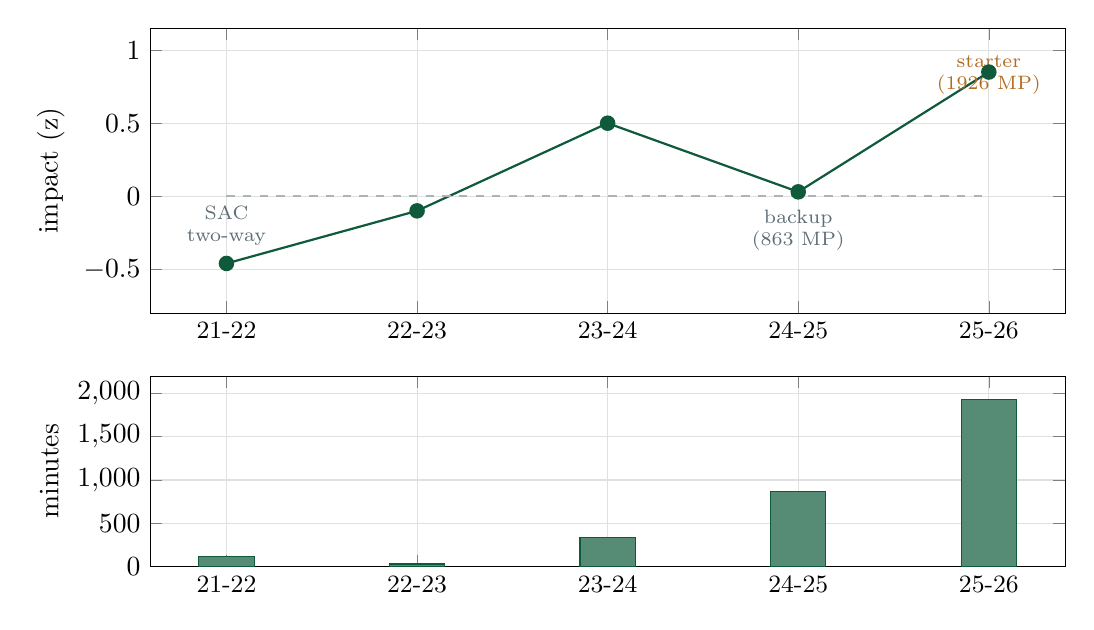
\begin{tikzpicture}
\begin{groupplot}[
  group style={group size=1 by 2, vertical sep=8mm},
  width=13.2cm, xtick=data,
  symbolic x coords={21-22,22-23,23-24,24-25,25-26},
  x tick label style={font=\small},
]
\nextgroupplot[height=5.2cm, ylabel={impact (z)},
  ymin=-0.8, ymax=1.15, ytick={-0.5,0,0.5,1},
  grid=major, grid style={fade!40},
  every axis plot/.append style={thick}]
\addplot[color=court, mark=*, mark size=2.4pt] coordinates
  {(21-22,-0.46) (22-23,-0.10) (23-24,0.50) (24-25,0.03) (25-26,0.85)};
\addplot[color=fade, dashed] coordinates {(21-22,0) (25-26,0)};
\node[font=\scriptsize, color=steel, anchor=south, align=center] at (axis cs:21-22,-0.40)
  {SAC\\ two-way};
\node[font=\scriptsize, color=steel, anchor=north, align=center] at (axis cs:24-25,-0.03)
  {backup\\ (863 MP)};
\node[font=\scriptsize, color=amberx, anchor=south, align=center] at (axis cs:25-26,0.63)
  {starter\\ (1926 MP)};
\nextgroupplot[height=4.0cm, ylabel={minutes}, ymin=0, ymax=2200,
  ytick={0,500,1000,1500,2000}, grid=major, grid style={fade!40}]
\addplot[ybar, bar width=20pt, fill=court!70, draw=court] coordinates
  {(21-22,120) (22-23,29) (23-24,333) (24-25,863) (25-26,1926)};
\end{groupplot}
\end{tikzpicture}
\caption{Five seasons: per-minute impact (top) and the role that finally arrived
(bottom). The 2024--25 dip is real --- his box value that year was ordinary --- and the
paper does not hide it.}
\label{fig:arc}
\end{figure}

Two mechanical details explain why the role took five years and why it should persist.
First, the classic young-big constraint --- fouling --- has receded on schedule: his foul
rate went from the 6th percentile in 2023--24 (a foul machine, unplayable in long
stretches) to the 24th, to the 31st. Coaches could not keep him on the floor before;
in 2025--26 they could. Second, his efficiency did not bend as the load grew.

\begin{figure}[h]
\centering
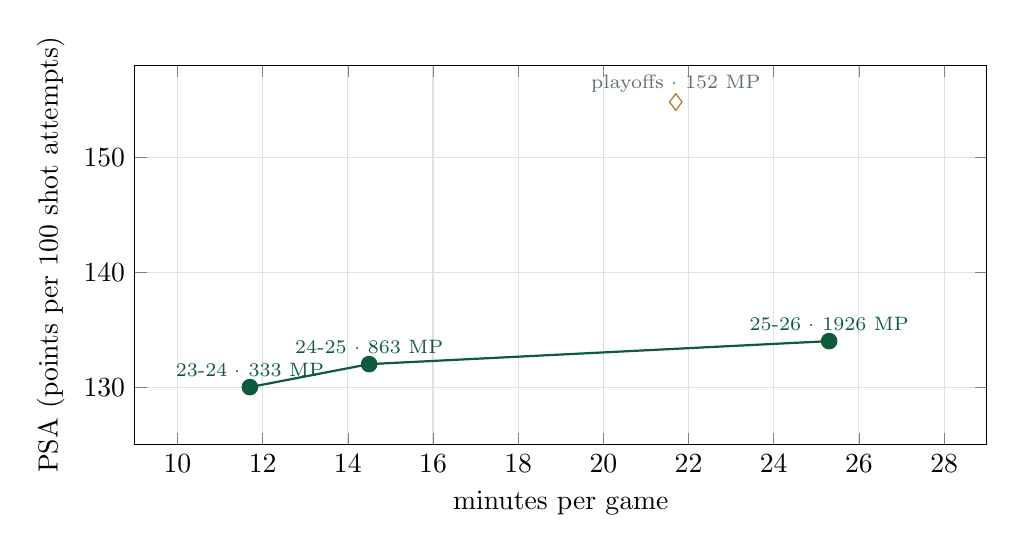
\begin{tikzpicture}
\begin{axis}[
  width=12.4cm, height=6.4cm,
  xlabel={minutes per game}, ylabel={PSA (points per 100 shot attempts)},
  xmin=9, xmax=29, ymin=125, ymax=158,
  grid=major, grid style={fade!40},
  every node near coord/.append style={font=\scriptsize},
]
\addplot[color=court, thick, mark=*, mark size=2.6pt,
  nodes near coords, point meta=explicit symbolic]
  coordinates {
    (11.7,130.0)[23-24 · 333 MP] (14.5,132.0)[24-25 · 863 MP] (25.3,134.0)[25-26 · 1926 MP]
  };
\addplot[only marks, mark=diamond, amberx, mark size=3.0pt,
  nodes near coords, point meta=explicit symbolic,
  every node near coord/.append style={color=steel}]
  coordinates {(21.7,154.8)[playoffs · 152 MP]};
\end{axis}
\end{tikzpicture}
\caption{The anti-fluke chart. \ctg{} scoring efficiency (PSA) against role size,
Boston regular seasons (labels show total bbref minutes). The normal pattern is a
downward slope --- bench bigs feast on easy minutes and regress when the role doubles.
Queta's minutes per game roughly doubled and his season workload grew nearly sixfold
(333 $\to$ 1{,}926 minutes), and the efficiency line went \emph{up}: 130 $\to$ 132
$\to$ 134, all 79th--87th percentile. The open diamond is the seven-game 2026 playoff
run (152 minutes, 97th percentile): a different competition environment on a small
sample, plotted separately and no part of the regular-season trend.}
\label{fig:path}
\end{figure}

\begin{table}[h]
\centering\small
\caption{The 2025--26 profile in \ctg{} percentiles (among bigs). This is what \#41 is
made of: elite finishing at real volume, elite offensive rebounding, real rim
protection, and the league's 17th-best filtered on/off among 1{,}500+ minute players.}
\begin{tabular}{lcc}
\toprule
Component & Value & Percentile \\
\midrule
Scoring efficiency (PSA) & 134.0 & 84th \\
eFG\% & 65.4\% & 86th \\
Rim accuracy & 75\% & 85th \\
Offensive rebound rate & 12.3\% & 79th \\
Block rate & 2.7\% & 79th \\
Defensive rebound rate & 19.9\% & 74th \\
Filtered on/off (raw) & $+8.6$ & \#17 of 158 league-wide \\
Turnover rate & 12.6\% & 55th \\
Foul rate & 4.4\% & 31st (up from 6th in '24) \\
Free-throw \% & 70.1\% & 41st \\
\bottomrule
\end{tabular}
\label{tab:profile}
\end{table}

\plainbox{Queta finally got starter minutes at 26 and his efficiency --- which usually
falls when a bench big's role doubles --- went up instead. He finishes like a top-10
center, crashes the offensive glass, blocks shots, and stopped fouling himself off the
floor. That's the whole trick: there is no empty-calorie stat propping him up.}

\section{Stress test I: shrink the shiny number}
\label{sec:noise}

The skeptic's first target should be that $+8.6$ on/off --- Boston was 8.6 points per
100 possessions better with Queta on the floor (garbage time excluded). On/off numbers
are notoriously unstable, so we measured the instability rather than argue about it.
For all 184 players with 1{,}000+ \ctg{} minutes in both 2024--25 and 2025--26, we
correlated their on/off across the two seasons (Figure~\ref{fig:onoff}):
\begin{equation}
r = 0.317 .
\label{eq:r}
\end{equation}
Call this what it is: \emph{cross-season persistence}. Only about a third of the
cross-player variation in filtered on/off carries into the following year. (Some of the
rest is measurement noise; some is genuine change in teammates, role, and scheme ---
both argue for discounting any single season's value.) Two technical notes a careful
reader deserves. First, $0.317$ is the Pearson correlation, but the season-to-season
standard deviations are nearly equal (5.66 vs.\ 5.74), so the least-squares slope,
$b = r \, s_{26}/s_{25} = 0.322$, is numerically the same discount. Second, there are
two defensible shrink targets. The textbook regression prediction shrinks toward the
qualifying pool's mean ($+1.2$):
\begin{equation}
\widehat{\text{on/off}} \;=\; 1.18 + 0.317\,(8.6 - 1.18) \;=\; +3.5 .
\label{eq:shrunkreg}
\end{equation}
The harsher convention shrinks toward zero:
\begin{equation}
\widehat{\text{on/off}}_{\text{harsh}} \;=\; r \times 8.6 \;=\; \mathbf{+2.7}.
\label{eq:shrunk}
\end{equation}
We test the claim against both, and quote the harsher one in the summary.

\begin{figure}[h]
\centering
\begin{tikzpicture}
\begin{axis}[
  width=11.8cm, height=7.6cm,
  xlabel={on/off, 2024--25}, ylabel={on/off, 2025--26},
  xmin=-16, xmax=18, ymin=-16, ymax=18,
  grid=major, grid style={fade!40},
  legend style={font=\small, at={(0.97,0.03)}, anchor=south east},
]
\addplot[only marks, mark=*, mark size=1.3pt, color=steel!70, opacity=0.55]
  table {onoff_pairs.dat};
\addplot[color=fade!60!black, dashed, thick, domain=-16:18] {x};
\addplot[color=court, thick, domain=-16:18] {1.18+0.322*(x-1.16)};
\addplot[only marks, mark=diamond*, amberx, mark options={fill=amberx}, mark size=4pt]
  coordinates {(-0.8,8.6)};
\node[font=\scriptsize, color=amberx, anchor=west] at (axis cs:0.2,9.6) {Queta};
\legend{184 players (1000+ MP both yrs), no regression ($y{=}x$), least-squares fit ($b{=}0.32$)}
\end{axis}
\end{tikzpicture}
\caption{How much of an on/off number persists into the next year? The cloud says:
about a third. The amber diamond is Queta --- his 2024--25 on/off (a $-0.8$ in his
backup season: 863 bbref minutes, 768 after \ctg{}'s garbage-time filter, too few to
qualify for the cloud) carried almost no information; his 2025--26 value is large but
must be discounted by \eqref{eq:shrunkreg}--\eqref{eq:shrunk} before you believe it.}
\label{fig:onoff}
\end{figure}

This is the paper attacking its own best exhibit, so state the result plainly --- and
the attack draws real blood. There are two coherent readings of ``on/off is mostly
noise,'' and they cut very differently. \emph{If every player's on/off is equally
unstable}, the discount changes nothing: \gravity{} uses on/off as a within-season
z-score, and shrinking an entire column toward its mean leaves every z-score --- and
every rank --- exactly where it was. \#41 is untouched. The skeptic's real claim must
therefore be sharper: that \emph{Queta's number specifically} is inflated relative to
his peers'. We tested that harshest reading by forcing his on/off input alone down to
the discounted values and re-running the entire 644-player pipeline. At the
regression value ($+3.5$) he lands at 57.2, \textbf{\#53}; at the toward-zero value
($+2.7$), 56.9, \textbf{\#55}. (Version 1 of this paper reported $\approx$\#48 here,
from a shortcut recomputation; the full re-run is the correct number, and it is worse
for us.) So the honest summary: under the harshest single-player discount, Queta slips
just \emph{outside} the top 50 --- the placement is carried mostly, but not entirely,
by the box profile of Table~\ref{tab:profile} (on/off is 14\% of the impact blend,
Appendix~\ref{app:spec}). The claim ``top-50 player'' narrows to the boundary. That is
precisely why Section~\ref{sec:predict} registers the forward bet at 75\% rather than
declaring the present tense settled.

\plainbox{Only about a third of a season's on/off carries into the next year --- we
measured it (r = 0.317, n = 184). If everyone's number is equally noisy, \#41 doesn't
move at all. If you believe Queta's alone is inflated --- the harshest reading --- he
lands \#53--55, just outside the claim. The bet was never resting on the shiny number,
but v2 owes you the truth that the harshest discount grazes it.}

\section{Stress test II: what happened to everyone like him}
\label{sec:comps}

The second attack: \emph{every} backup-turned-starter big has one shiny efficient
season; most regress. Rather than argue by anecdote, we built the cohort. From six
seasons of league data (2019--20 through 2024--25), we extracted every big-man season
matching Queta's 2025--26 statistical silhouette --- usage $\le 19$, WS/48 $\ge .190$,
TS $\ge .630$, block rate $\ge 1.8\%$, 900--2{,}500 minutes, age $\le 28$ --- and
followed each into the next season. There are 33 such \emph{seasons}, from 22 distinct
players (a distinction the analysis below keeps honest), and the family is exactly who
you'd hope: Gobert, Robert Williams, Jarrett Allen (four times), Zubac, Hartenstein,
Gafford, Claxton, Kessler, Duren --- and, three times, Mitchell Robinson.

\begin{table}[h]
\centering\small
\caption{Selected comparables (of 33): elite-efficiency, low-usage big seasons and what
happened next. Full criteria in text; IMPACT in z units, Pct = next-season percentile
among 1{,}000+ minute players.}
\begin{tabular}{llcccccc}
\toprule
Year & Player & Age & MP & IMPACT & Next MP & Next IMPACT & Next Pct \\
\midrule
2020--21 & Robert Williams & 23 & 985 & $+1.66$ & 1804 & $+1.48$ & 95 \\
2024--25 & Jalen Duren & 21 & 2034 & $+1.02$ & 1976 & $+1.60$ & 97 \\
2019--20 & Rudy Gobert & 27 & 2333 & $+1.12$ & 2187 & $+1.38$ & 94 \\
2023--24 & Daniel Gafford & 25 & 1815 & $+0.89$ & 1226 & $+1.32$ & 95 \\
2024--25 & Jarrett Allen & 26 & 2296 & $+1.26$ & 1519 & $+0.88$ & 88 \\
2023--24 & Isaiah Hartenstein & 25 & 1896 & $+0.87$ & 1590 & $+0.86$ & 84 \\
2021--22 & Isaiah Hartenstein & 23 & 1216 & $+1.34$ & 1626 & $-0.16$ & 42 \\
2022--23 & Walker Kessler & 21 & 1703 & $+0.89$ & 1493 & $+0.24$ & 67 \\
2022--23 & Nic Claxton & 23 & 2271 & $+0.96$ & 2116 & $+0.38$ & 73 \\
2021--22 & Mitchell Robinson & 23 & 1848 & $+0.75$ & 1591 & $+0.63$ & 82 \\
2019--20 & Mitchell Robinson & 21 & 1412 & $+1.02$ & 853 & $+0.34$ & 69 \\
2020--21 & Enes Freedom & 28 & 1758 & $+0.39$ & 411 & $-0.23$ & 38 \\
\midrule
\multicolumn{8}{l}{\textbf{All 33 seasons:} median next-season percentile \textbf{75th};
$\ge$80th: \textbf{45\%}; $\ge$85th (top-50-caliber): \textbf{39\%}} \\
\multicolumn{8}{l}{\textbf{22 unique players}, counting each once: $\ge$85th
\textbf{32\%}, median percentile 73rd (clustered player-means agree)} \\
\multicolumn{8}{l}{median impact regresses $+0.89 \to +0.47$; median minutes change
$\mathbf{-146}$; 55\% kept $\ge$90\% of their minutes, 42\% grew} \\
\bottomrule
\end{tabular}
\label{tab:comps}
\end{table}

\begin{figure}[h]
\centering
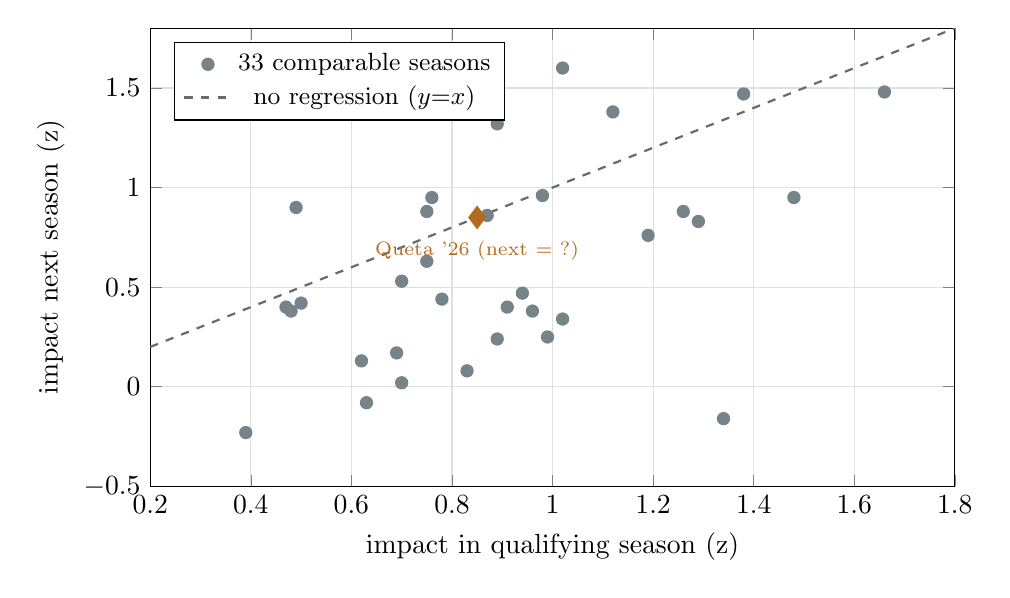
\begin{tikzpicture}
\begin{axis}[
  width=11.8cm, height=7.4cm,
  xlabel={impact in qualifying season (z)}, ylabel={impact next season (z)},
  xmin=0.2, xmax=1.8, ymin=-0.5, ymax=1.8,
  grid=major, grid style={fade!40},
  legend style={font=\small, at={(0.03,0.97)}, anchor=north west},
]
\addplot[only marks, mark=*, mark size=2.2pt, color=steel!85]
  coordinates {(1.12,1.38) (1.02,0.34) (0.99,0.25) (0.94,0.47) (0.78,0.44) (0.70,0.02)
  (0.48,0.38) (1.66,1.48) (1.38,1.47) (0.49,0.90) (0.47,0.40) (0.39,-0.23) (1.48,0.95)
  (1.34,-0.16) (1.29,0.83) (1.19,0.76) (0.75,0.63) (0.70,0.53) (0.50,0.42) (0.96,0.38)
  (0.89,0.24) (0.83,0.08) (0.76,0.95) (0.69,0.17) (0.63,-0.08) (0.62,0.13) (0.98,0.96)
  (0.91,0.40) (0.89,1.32) (0.87,0.86) (1.26,0.88) (1.02,1.60) (0.75,0.88)};
\addplot[color=fade!60!black, dashed, thick, domain=0.2:1.8] {x};
\addplot[only marks, mark=diamond*, amberx, mark options={fill=amberx}, mark size=4pt]
  coordinates {(0.85,0.85)};
\node[font=\scriptsize, color=amberx, anchor=north] at (axis cs:0.85,0.78)
  {Queta '26 (next = ?)};
\legend{33 comparable seasons, no regression ($y{=}x$)}
\end{axis}
\end{tikzpicture}
\caption{Regression to the mean, drawn honestly. Most dots sit below the dashed line:
seasons like this usually give some value back. But the floor is high --- three-quarters
of the cohort remained above the league median, and two in five delivered a
top-50-caliber (85th+ percentile) follow-up.}
\label{fig:comps}
\end{figure}

Two robustness checks, because a critic should ask whether the criteria were tuned ---
consciously or not --- to produce a flattering family. First, \emph{players versus
seasons}: repeat careers (Allen four times, Robinson three) give some players multiple
votes. Counting each player once drops the top-50-caliber follow-up rate from 39\% to
32\%; clustering outcomes by player gives the same answer. The honest base rate is
``roughly one in three,'' and we carry both figures forward. Second, \emph{the
cutoffs}: Table~\ref{tab:sens} re-runs the engine varying one criterion at a time.

\begin{table}[h]
\centering\small
\caption{Cohort sensitivity: one cutoff varied at a time. The follow-up rate never
falls below 38\%, and the strictest efficiency cut \emph{raises} it --- the criteria
were not tuned to flatter the conclusion.}
\begin{tabular}{lcccc}
\toprule
Variation & Seasons & Unique players & $\ge$85th pct rate & Median next pct \\
\midrule
As published & 33 & 22 & 39\% & 75 \\
TS $\ge .620$ (looser) & 33 & 22 & 39\% & 75 \\
TS $\ge .640$ (stricter) & 29 & 18 & 41\% & 78 \\
WS/48 $\ge .175$ (looser) & 41 & 25 & 39\% & 74 \\
WS/48 $\ge .205$ (stricter) & 20 & 13 & 55\% & 86 \\
Minutes $\ge 1{,}100$ & 29 & 20 & 38\% & 75 \\
Usage $\le 20$ & 35 & 22 & 40\% & 75 \\
Block rate $\ge 1.5\%$ & 33 & 22 & 39\% & 75 \\
\bottomrule
\end{tabular}
\label{tab:sens}
\end{table}

The base rates give the skeptic real ammunition --- the median comparable gave back
about half his impact z, and minutes \emph{shrank} more often than grew --- and they
give the bull real support: 32--39\% of the cohort (by player and by season) posted a
top-50-caliber next season, the rate survives every cutoff variation we tested, and
the family's floor is remarkably high. Two situational facts then push Queta above the
cohort median. Most comparables were backups fighting for a role (Kornet,
Jackson-Davis, Clarke); Queta is the \emph{incumbent starter} on a 56-win team. And no
comparable had his team commit \$56M in July. Base rate roughly one in three,
situation-adjusted: higher --- and Section~\ref{sec:predict} must now say by how much,
and why.

\plainbox{We found the 33 seasons (22 players) statistically most like 2025--26 Queta
over the last six years. Most gave a little back the next season --- but roughly one in
three players (two in five season-weighted) delivered a top-50-level year, the rate
survives every threshold we varied, and unlike most of them, Queta enters next season
with the starting job, a new contract, and a 56-win team around him.}

\section{The Robinson question}
\label{sec:robinson}

The strongest objection isn't statistical, it's transactional: on July 6 Boston signed
Mitchell Robinson --- the champion Knicks' rim protector --- for three years and \$47.4M.
If Robinson takes 24 minutes a night, the bear case writes itself.

Three replies, in declining order of hardness. \emph{First}, the revealed preference:
Boston extended Queta for \$56M days \emph{after} the Robinson deal, and beat reporting
projects Queta to open as the starter, with something like an even split behind him.
Teams do sometimes pay two centers for depth, insurance, or matchups, so the contracts
do not fix his role --- what they establish is narrower but real: Boston values Queta
at starter money while holding better information than any public model, and plans to
play him. \emph{Second}, Robinson's own availability record is the worst in the
comparables family --- 60+ games in only three of his last seven seasons, and he appears
in Table~\ref{tab:comps} three times precisely because he keeps posting elite fragments
(853, 768, 1{,}591 minutes follow-ups); planning a center rotation around Robinson's
health has broken repeatedly for a decade. \emph{Third}, the tide: Jayson Tatum returns
for a full season. His early post-Achilles evidence is encouraging --- 16 regular-season
games plus a seven-game playoff series at an 8.9 BPM --- though samples that size cannot
yet certify the recovery. It raises every Celtic's context --- and Queta's playoff
series alongside him (.767 TS) was his best basketball of the year. The honest version of the Robinson signing is a minutes
tax on the bear case, not a refutation: it lowers Queta's floor scenario from ``starter
by default'' to ``starter by performance,'' which --- given Section~\ref{sec:comps} ---
is a bet the data supports.

\section{The prediction}
\label{sec:predict}

Now the arithmetic --- with the division of labor stated plainly, because it is the
part of this paper most deserving of scrutiny. The two-year \gravity{} machinery
(Appendix~\ref{app:spec}) converts any assumed 2026--27 performance level and workload
into a score; the top-50 cutoff in the July 2026 distribution is \textbf{57.4}.
\emph{Those scores are model output.} The four scenarios and their weights are
\emph{not}: they are editorial judgments, and the subsection below anchors each one to
an observable rate so the reader can price the judgment rather than take it.

\begin{table}[h]
\centering\small
\caption{Four futures, weighted. Impact is 2026--27 per-minute value in z units --- his
2025--26 was $+0.97$ under current \gravity{} (which includes on/off) and $+0.85$ under
\gravity-RS (the no-on/off variant used in Table~\ref{tab:career} and the comparables
engine); the blend automatically carries 2025--26 forward as the trailing season.
Scores: model. Weights: authors.}
\begin{tabular}{lccccccl}
\toprule
Scenario & Weight & Impact & MP & GP & Score & Top-50? & Reading \\
\midrule
Bust: loses the job & 15\% & $+0.30$ & 1000 & 50 & 53.8 & no & Robinson takes over \\
Bear: even timeshare & 25\% & $+0.75$ & 1450 & 62 & 58.1 & \emph{barely} & regression + split \\
Base: holds the job & 40\% & $+1.00$ & 2000 & 74 & 62.3 & yes (\#23--27) & 2025--26 continues \\
Bull: consolidation & 20\% & $+1.25$ & 2300 & 76 & 66.9 & yes (\#10--13) & comps' top tercile \\
\midrule
\multicolumn{8}{l}{$P(\text{top-50}) \approx 0.25{\times}0.6 + 0.40 + 0.20 =
\mathbf{0.75}$ \quad (bear counted 60\%, being borderline --- a judgment, like the weights)} \\
\multicolumn{8}{l}{$P(\text{top-25}) \approx 0.40{\times}0.5 + 0.20 = \mathbf{0.40}$} \\
\bottomrule
\end{tabular}
\label{tab:scenarios}
\end{table}

\begin{figure}[h]
\centering
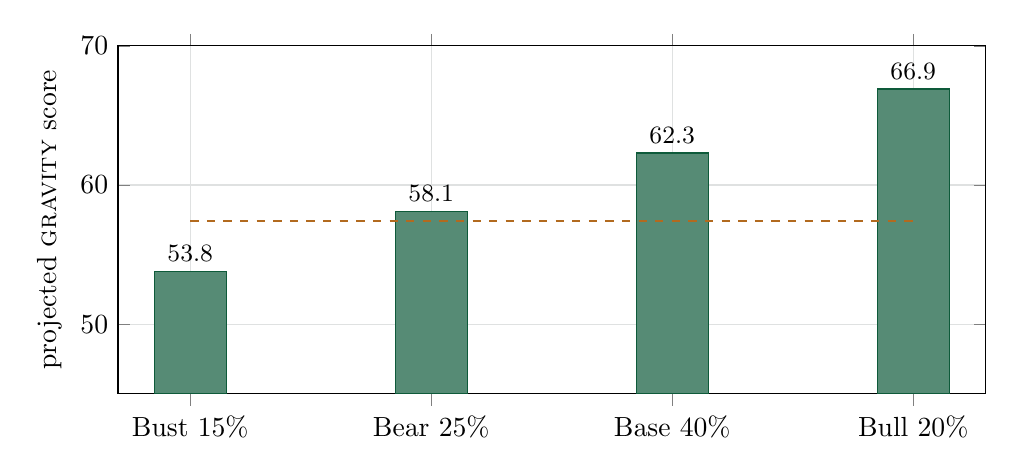
\begin{tikzpicture}
\begin{axis}[
  width=12.6cm, height=6.0cm, ybar, bar width=26pt,
  symbolic x coords={Bust 15\%, Bear 25\%, Base 40\%, Bull 20\%},
  xtick=data, ymin=45, ymax=70, ylabel={projected \gravity{} score},
  grid=major, grid style={fade!40},
]
\addplot[fill=court!70, draw=court, nodes near coords,
  every node near coord/.append style={font=\small}] coordinates
  {(Bust 15\%,53.8) (Bear 25\%,58.1) (Base 40\%,62.3) (Bull 20\%,66.9)};
\addplot[color=amberx, thick, dashed, sharp plot] coordinates
  {(Bust 15\%,57.4) (Bull 20\%,57.4)};
\end{axis}
\end{tikzpicture}
\caption{The bet, drawn. The dashed amber line is the top-50 cutoff in the July 2026
distribution (57.4). Three of four scenarios clear it; under our weights the assigned
probability is about 75\%.}
\label{fig:scen}
\end{figure}

\subsection*{Where the weights come from}

The move from a one-in-three base rate to a 75\% forecast is the least-supported leap a
skeptic will find in this paper, so here is each weight against the observable that
disciplines it. \textbf{Bust, 15\%:} losing the job outright requires Mitchell Robinson
to be simultaneously healthy and clearly better --- Robinson has reached 60 games in
three of his last seven seasons ($\approx$43\%), and the incumbent he must displace was
just extended at starter money; the joint event deserves a weight well below either
margin. \textbf{Bear, 25\%:} the cohort says roles shrink more often than they grow
(median $-146$ minutes; only 42\% grew), so a timeshare is the modal downside and gets
the second-largest weight. \textbf{Base, 40\%:} 55\% of comparables kept at least 90\%
of their minutes, and Queta holds two advantages most of them lacked --- incumbency and
the contract --- so ``2025--26 repeats'' is the single most likely outcome, weighted
slightly below the naked retention rate out of respect for Robinson. \textbf{Bull,
20\%:} one third of the cohort landed in the top tercile of follow-ups; we haircut that
for the crowded frontcourt. These anchors discipline the weights; they do not compute
them. A reader who rejects every situational adjustment should simply hold the cohort
rate --- roughly one in three --- and the distance between that number and 75\% is
exactly the size of the bet this paper places on incumbency, the extension, Robinson's
availability record, and Tatum's return.

Note also what makes the claim robust: it does not require a leap. The base case is
simply \emph{2025--26 happening again} --- same job, same efficiency, ordinary
regression --- and it lands at \#23--27, comfortably inside the claim. The prediction
fails only if Robinson takes the job outright or the season-scale regression lands in
the worst tercile of the comparables. \textbf{Falsification criteria, on the record:}
in the July 2027 edition of ``The 644,'' computed by this same specification, Queta at
\#50 or better scores as a win; below \#70 as a clean miss. The Ledger's registered
middle band (\#51--70, originally labeled a ``push'') stands as registered, but v2
tightens the grading against ourselves: \emph{the claim is ``top-50,'' so \#51 is a
failure}. A \#51--70 finish will be graded a \textbf{near miss} --- a failed prediction
owing a diagnosis, not partial credit --- and the binary verdict, top-50 or not, is
what the July 2027 audit will headline.

\plainbox{The bet: we assign about 75\% to Queta being a top-50 player in next July's
ranking, and 2-in-5 to top-25 --- the model prices the scenarios, we chose the weights,
and the anchors above show our work. It's not a moonshot claim; it just requires this
season to mostly repeat. We wrote down in advance exactly what counts as being wrong,
and \#51 counts.}

\section{Conclusion}

The Queta problem narrows under measurement to something bettable. A \#41 ranking that
looks like a model glitch turns out to rest on the most trustworthy statistics in the
sport --- hundreds of finished possessions at 85th-percentile efficiency, elite
offensive rebounding, real rim protection --- and the two best attacks we could mount
on it leave marks without landing: discounting his on/off by its measured cross-season
persistence ($r = 0.317$) leaves \#41 untouched if the discount applies to everyone,
and puts him at \#53--55 under the harshest reading that his number alone is inflated;
the 33-season, 22-player comparables cohort puts the base rate of a top-50-caliber
follow-up at roughly one in three, robust to every cutoff we varied, before counting
his incumbency, his new contract, or Tatum's return. The model prices the futures; the
weights that turn those prices into a 75\% forecast are ours, anchored and argued in
Section~\ref{sec:predict}. Boston's own front office, holding better information than
any public model, paid \$56 million for a related conclusion. The market will grade us
in twelve months.

\section*{Revision note (v2, July 11, 2026)}
Following a detailed external review, this version separates model output from
editorial judgment and corrects one number. (1) The scenario probabilities were
presented as \gravity{} output; they are the authors' weights applied to \gravity{}
scores, and a new subsection anchors each weight to an observable rate. (2) ``On/off is
two-thirds noise'' overstated what a cross-season correlation shows; the language now
says \emph{persistence}, reports the regression slope alongside $r$ (they are
numerically equal here), and gives both shrink targets. (3) The shrunk-on/off
counterfactual was corrected: a full re-run of the 644-player pipeline gives \#53--55,
not the $\approx$\#48 a shortcut recomputation produced in v1 --- the harshest
single-player discount moves Queta just outside the top 50, and the paper now says so;
the uniform-discount case (ranks unchanged) was added for the same honesty. (4) The
comparables cohort now discloses 33 seasons from 22 unique players, reports per-player
rates (32\% vs.\ 39\%), and adds a cutoff-sensitivity table. (5) The grading of the
registered forecast was tightened against ourselves: \#51--70 will be graded a near
miss, not a push. (6) Figure~\ref{fig:path} now labels minutes and separates the
playoff sample from the regular-season trend; minutes sources (bbref vs.\ \ctg{}
filtered) are labeled throughout; the Robinson-contract and Tatum-recovery inferences
were softened to what the evidence supports. The registered forecast itself --- 75\%
top-50, 40\% top-25, scored July 2027 --- is unchanged: that is the bet, and moving it
after registration is the one revision this publication does not allow.

\appendix
\section{The GRAVITY specification (compact)}
\label{app:spec}

Identical to Research Note No.\ 1 and the July 10, 2026 ``The 644'' ranking (v3). For
season $y$, minutes-weighted moments define clipped z-scores
$z_k(i) = \mathrm{clip}((x_k(i)-\mu_k)/\sigma_k, \pm 4)$. Components: efficiency-under-load
$(\mathrm{TS}-\mu_{\mathrm{TS}})\cdot 100\cdot(\mathrm{clip}(\mathrm{USG},8,36)/20)^{0.7}$;
creation $\mathrm{AST\%}-0.55\,\mathrm{TOV\%}$; load $\mathrm{USG}+0.4\,\mathrm{AST\%}$;
stocks $2\,\mathrm{STL\%}+1.2\,\mathrm{BLK\%}$; rim pressure; volume (pts/100). Skill
blend $S = 0.27 z_{\text{vol}} + 0.19 z_{\text{eff}} + 0.22 z_{\text{crea}} + 0.09
z_{\text{load}} + 0.10 z_{\text{stk}} + 0.05 z_{\text{reb}} + 0.08 z_{\text{rim}}$.
Season impact
\begin{equation}
I_y = \bigl[0.44 z_{\mathrm{BPM}} + 0.12 z_{\mathrm{WS/48}}
+ 0.14 z(\Delta_{\text{on/off}} \min(1, m/2400)) + 0.30 S\bigr] \sqrt{\min(1, m/800)},
\label{eq:impact}
\end{equation}
blended across two seasons with minute-proportional weights ($0.75$ on the recent
year), shrunk toward replacement $\rho = -1.9$ with credibility
$c = \sqrt{\min(M, 2200)/2200}$, adjusted for playoff evidence and age, then discounted
by availability $A = 0.78 + 0.22\min(1, (0.7 g_y + 0.3 g_{y-1})/55)$, role size
$\Phi = 0.62 + 0.38 \min(1, \mathrm{mpg}^{*}/32)$, and documented injuries
$J \in [0.78, 1]$. Final scale $G = 50 + 15[\rho + (\tilde{R}+\pi+\alpha-\rho) A \Phi J]$.
The historical variant \gravity-RS (used for Table~\ref{tab:career} and the comparables
engine) deletes the on/off term and renormalizes to
$[0.533 z_{\mathrm{BPM}} + 0.133 z_{\mathrm{WS/48}} + 0.333 S']\sqrt{\min(1, m/800)}$.

\subsection*{Data and forecast registration}
Basketball-Reference league tables 2019--20 through 2025--26 ($\approx$4{,}400
player-seasons); Cleaning the Glass subscriber database (filtered on/off, shot zones,
foul and rebounding rates; player page 4902), accessed July 10, 2026. The on/off cross-season
persistence estimate uses all 184 players with 1{,}000+ \ctg{} minutes in both 2024--25
and 2025--26. No external rankings or projections were consulted. Prediction registered
July 10, 2026; to be scored against the July 2027 ``The 644.''

\begin{thebibliography}{9}
\bibitem{bbref} Basketball-Reference.com, league tables, accessed July 10, 2026.
\bibitem{ctg} Cleaning the Glass, player and leaders tables (subscription).
\url{https://cleaningtheglass.com/stats/player/4902}
\bibitem{start} ``Why Neemias Queta is the Celtics' starting center for 2025--26,''
Yahoo Sports / NBC Sports Boston, October 2025.
\bibitem{ext} ``Celtics sign Neemias Queta to \$56 million extension after Mitchell
Robinson addition,'' Yahoo Sports, July 2026.
\bibitem{robinson} ``Mitchell Robinson joining Celtics on 3-year, \$47.4M deal,''
NBA.com / Hoops Rumors, July 6, 2026.
\bibitem{n1} \gravity{} Research Note No.\ 1, ``The Rise and Fall of Ja Morant,''
July 10, 2026.
\end{thebibliography}

\end{document}
